\documentclass[../main]{subfiles}
\newcommand*\circled[1]{\tikz[baseline=(char.base)]{
            \node[shape=circle,draw,inner sep=1pt] (char) {#1};}}
    \begin{document}
    \setcounter{secnumdepth}{2}
    \chapter{提案手法}
        \section{提案手法の概要}
        本研究は,全天球カメラから取得した画像に基づき,通路認識を行う手法の検証を行う.ここでいう通路認識とは,画像中に通路があるかどうかを検出するだけでなく,
        画像中に通路がある場合,その通路がどのタイプに属するのかといった,通路の特徴を抽出することである.また,本研究で扱う通路のタイプは以下の8種類であり,
        それぞれの図を\fref{figure::new_aisle_type}に示す.\\\\
         \circled{1}一本道(straight)\\
         \circled{2}行き止まり(dead end)\\
         \circled{3}右のみ曲がれる角(right)\\
         \circled{4}左のみ曲がれる角(left)\\
         \circled{5}十字路(cross)\\
         \circled{6}右に曲がれる三叉路(3-way junction\_right)\\
         \circled{7}左に曲がれる三叉路(3-way junction\_left)\\
         \circled{8}突き当たりの三叉路(3-way junction\_center)
       
        \vskip\baselineskip
        \vskip\baselineskip

        本手法の通路認識の流れを\fref{figure::proposed_method_fig}に示す.
        まず,全天球カメラにより取得したRGBの画像配列データをYOLOの入力とし,出力されたバウンディングボックスとクラス確率の情報をもとに
        画像中に通路があるかどうかを検出する.画像中に通路が検出された場合,通路の座標位置に基づき,通路のタイプを決定する.

        %8タイプの通路の画像例
        \begin{figure}[H]
            \centering
            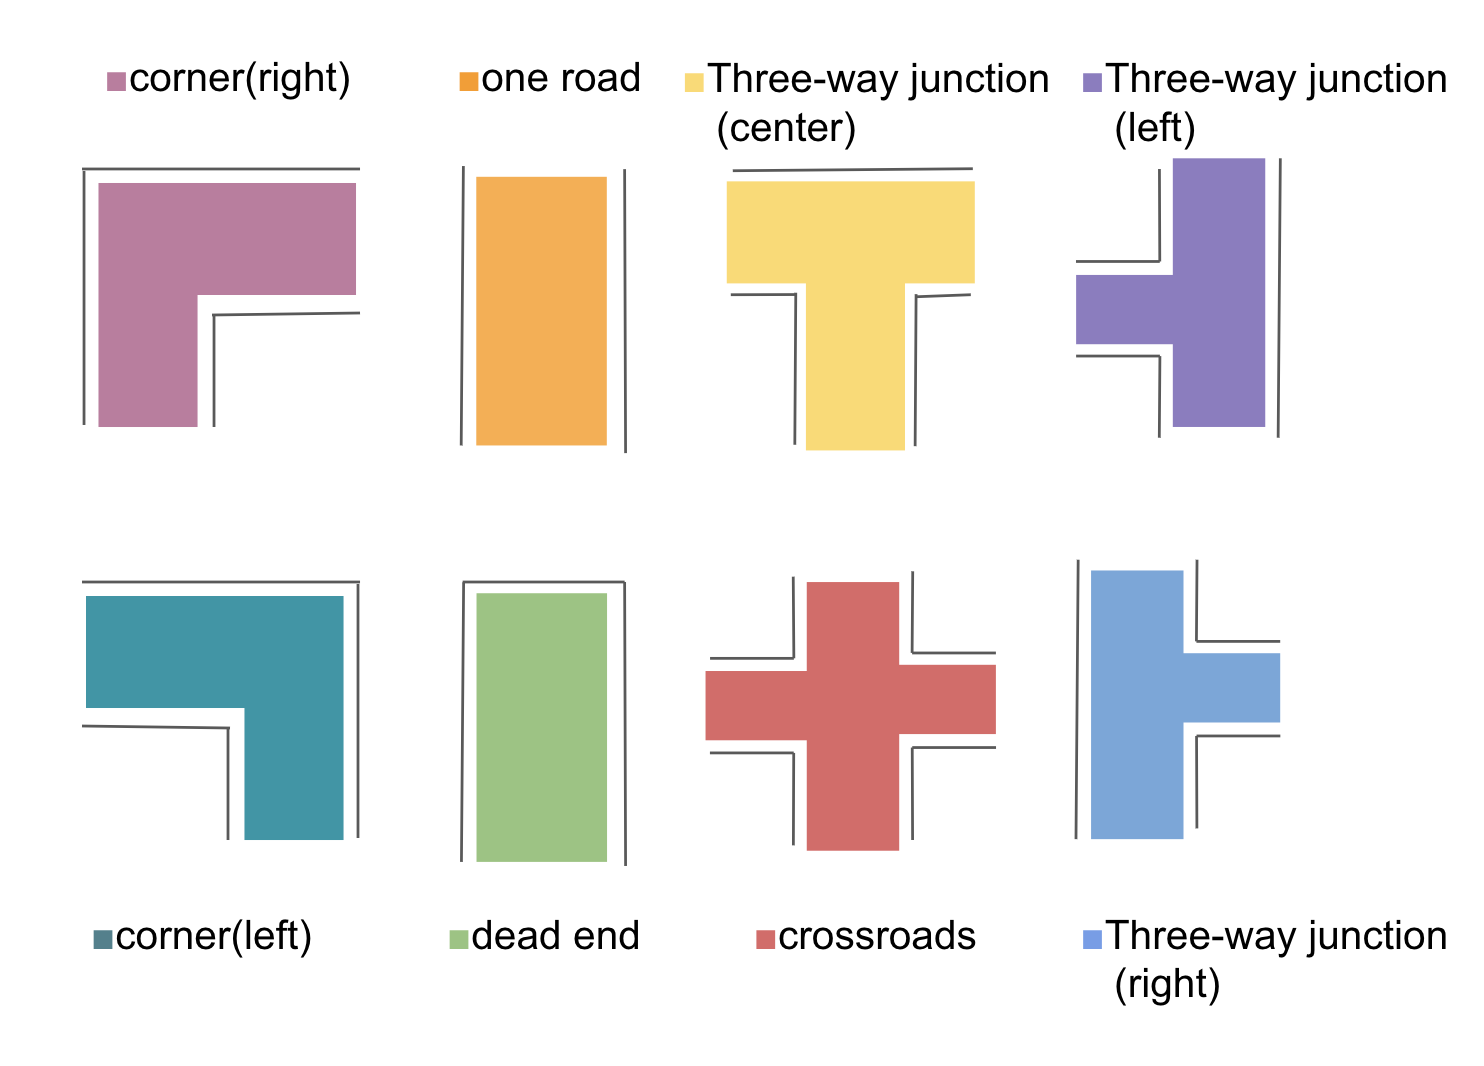
\includegraphics[width=10cm]{../images/new_aisle_type.png}
            \caption{Type of passage.}
            \label{figure::new_aisle_type}
        \end{figure}
        
        %提案手法の簡単な例
        \begin{figure}[H]
            \centering
            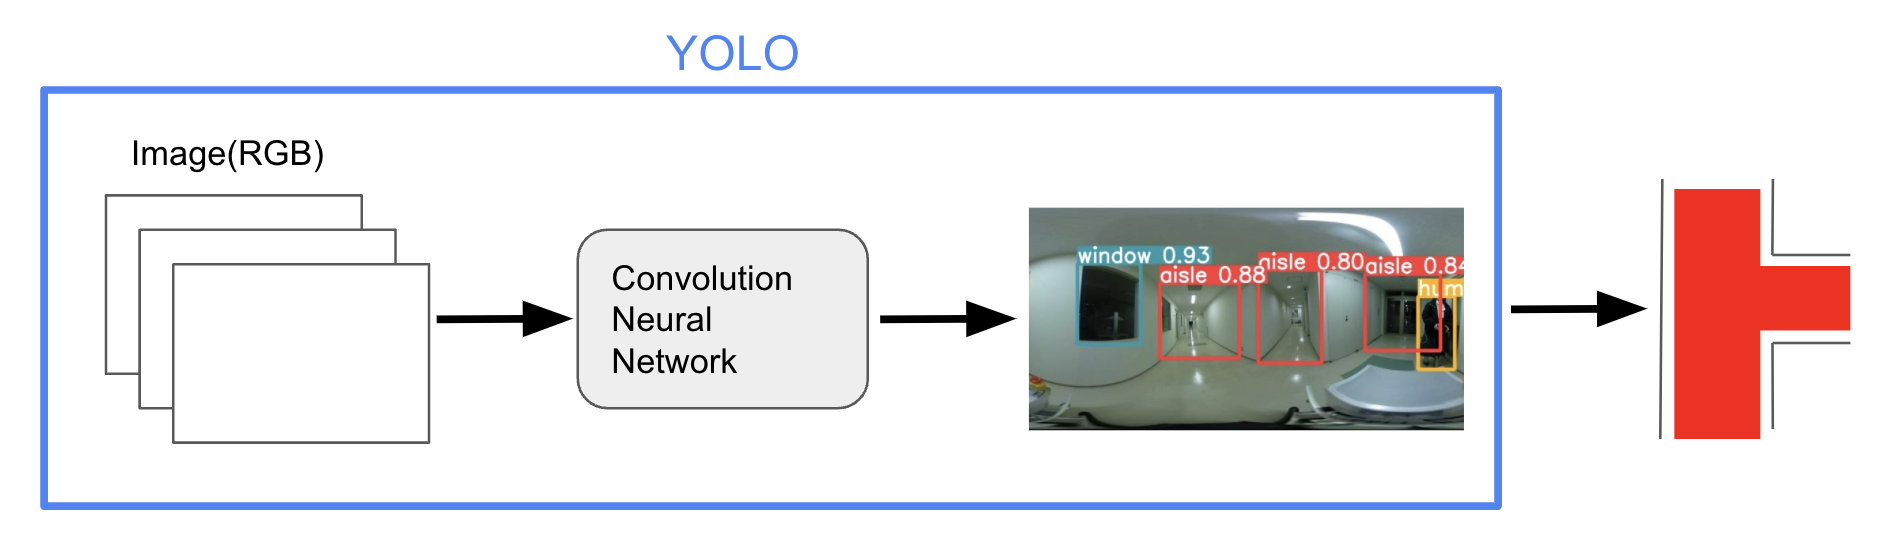
\includegraphics[width=15cm]{../images/proposed_method2.png}
            \caption{Flow of passage recognition method.}
            \label{figure::proposed_method_fig}
            この例では,YOLOの出力した画像から通路が3つ検出されている.\\
            また,通路はロボットに対して前方,後方,右手側に検出されているため,\\
            通路のタイプは\circled{6}右に曲がれる三叉路であるということがわかる.
        \end{figure}

        \newpage

        \section{画像の前処理}
        全天球カメラで取得した画像は通常,\fref{figure::no_proc}に示すように,カメラの正面が画像の中心となり,真後ろは画像の左端と右端で見切れてしまう.
        そこで,カメラに対する正面,真後ろ,真横(左右)にくる通路が見切れないように,YOLOに入力する前の段階で画像の前処理を行う.
        
        そこで,\fref{subfigure::preproc}に示すような画像の前処理を行なった.この処理では,320*640の全天球カメラ画像の左端を切り取り,
        右端に貼り付けるということを行なった.
        
        %画像の前処理の例
        \begin{figure}[htbp]
          \centering
           \subfigure[no processing image]{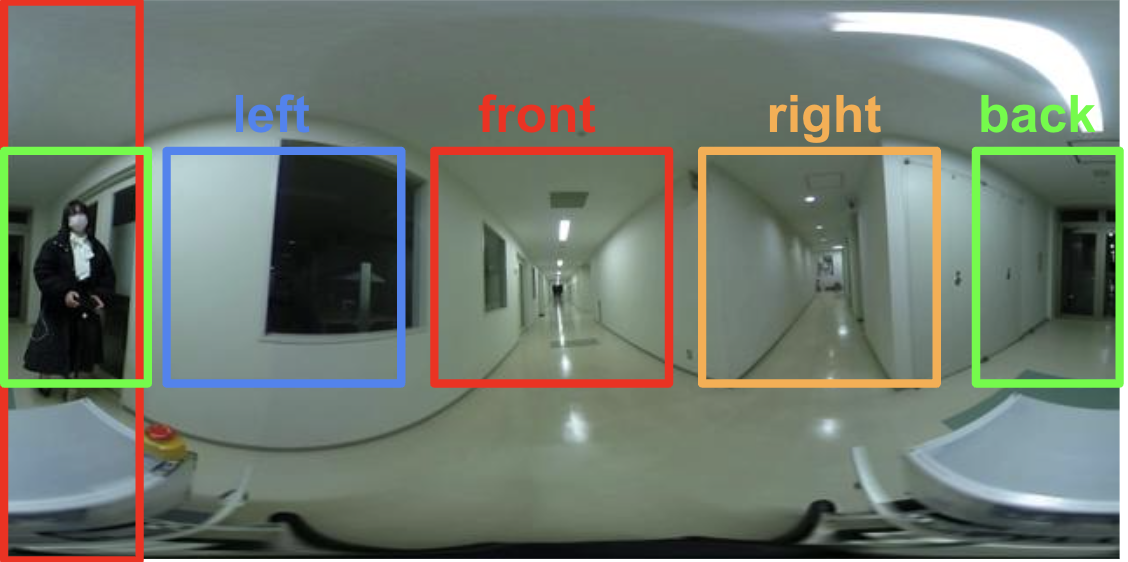
\includegraphics[height=4cm]{../images/no_processing.png}
           \label{subfigure::no_proc}}
           \subfigure[preprocessing image]{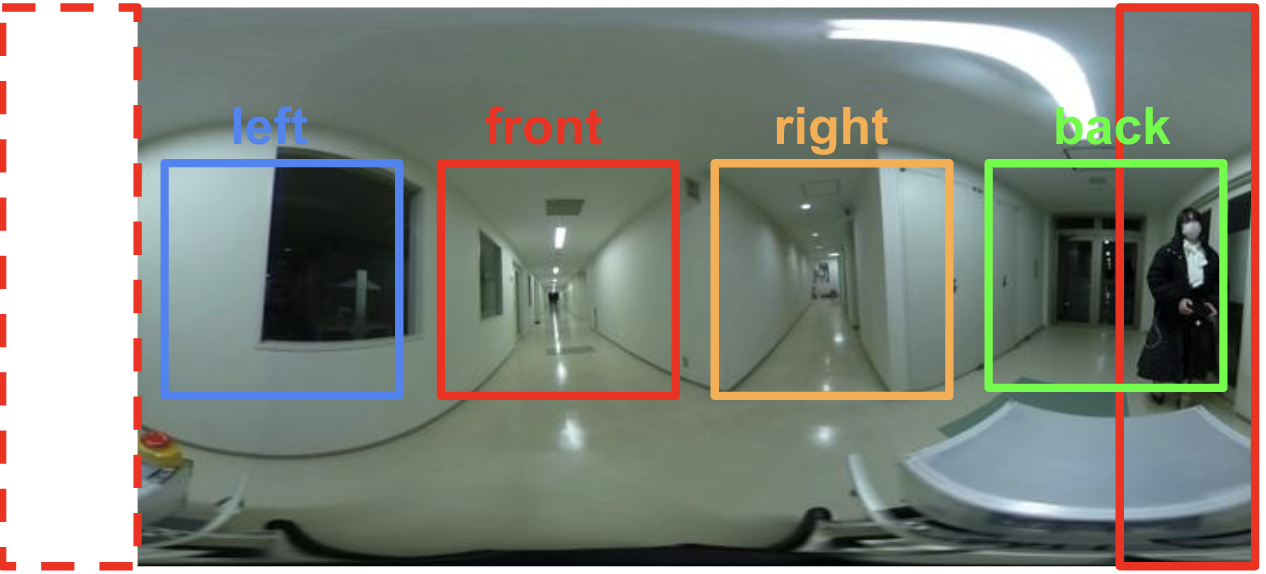
\includegraphics[height=4cm]{../images/after_processing.png}
           \label{subfigure::preproc}}
           \caption{Preprocessing of spherical camera images}
           \label{figure::proc_exp}
        \end{figure}
        
        \newpage

        \section{YOLOのデータセット作成}
        YOLOのモデル作成のため,自作のデータセットにより学習を行う.学習に使うデータは津田沼キャンパス2号館3階で収集した.
        また,データセットの一例を\fref{figure::dataset_fig}に示す.また,データセットのクラスは\tref{table::datasets_table}の11クラスで設定した.
        先行研究では,8つの形状タイプの通路の認識を行なったため,本研究でも先行研究と同様の通路認識を行う.
        次に,YOLOの出力として得られた通路の情報に基づき,を参考にし,画像中の通路が認識された箇所を場合分けし,通路の形状を決定する.

        %自作データセットの画像例
        \begin{figure}[H]
         \centering
         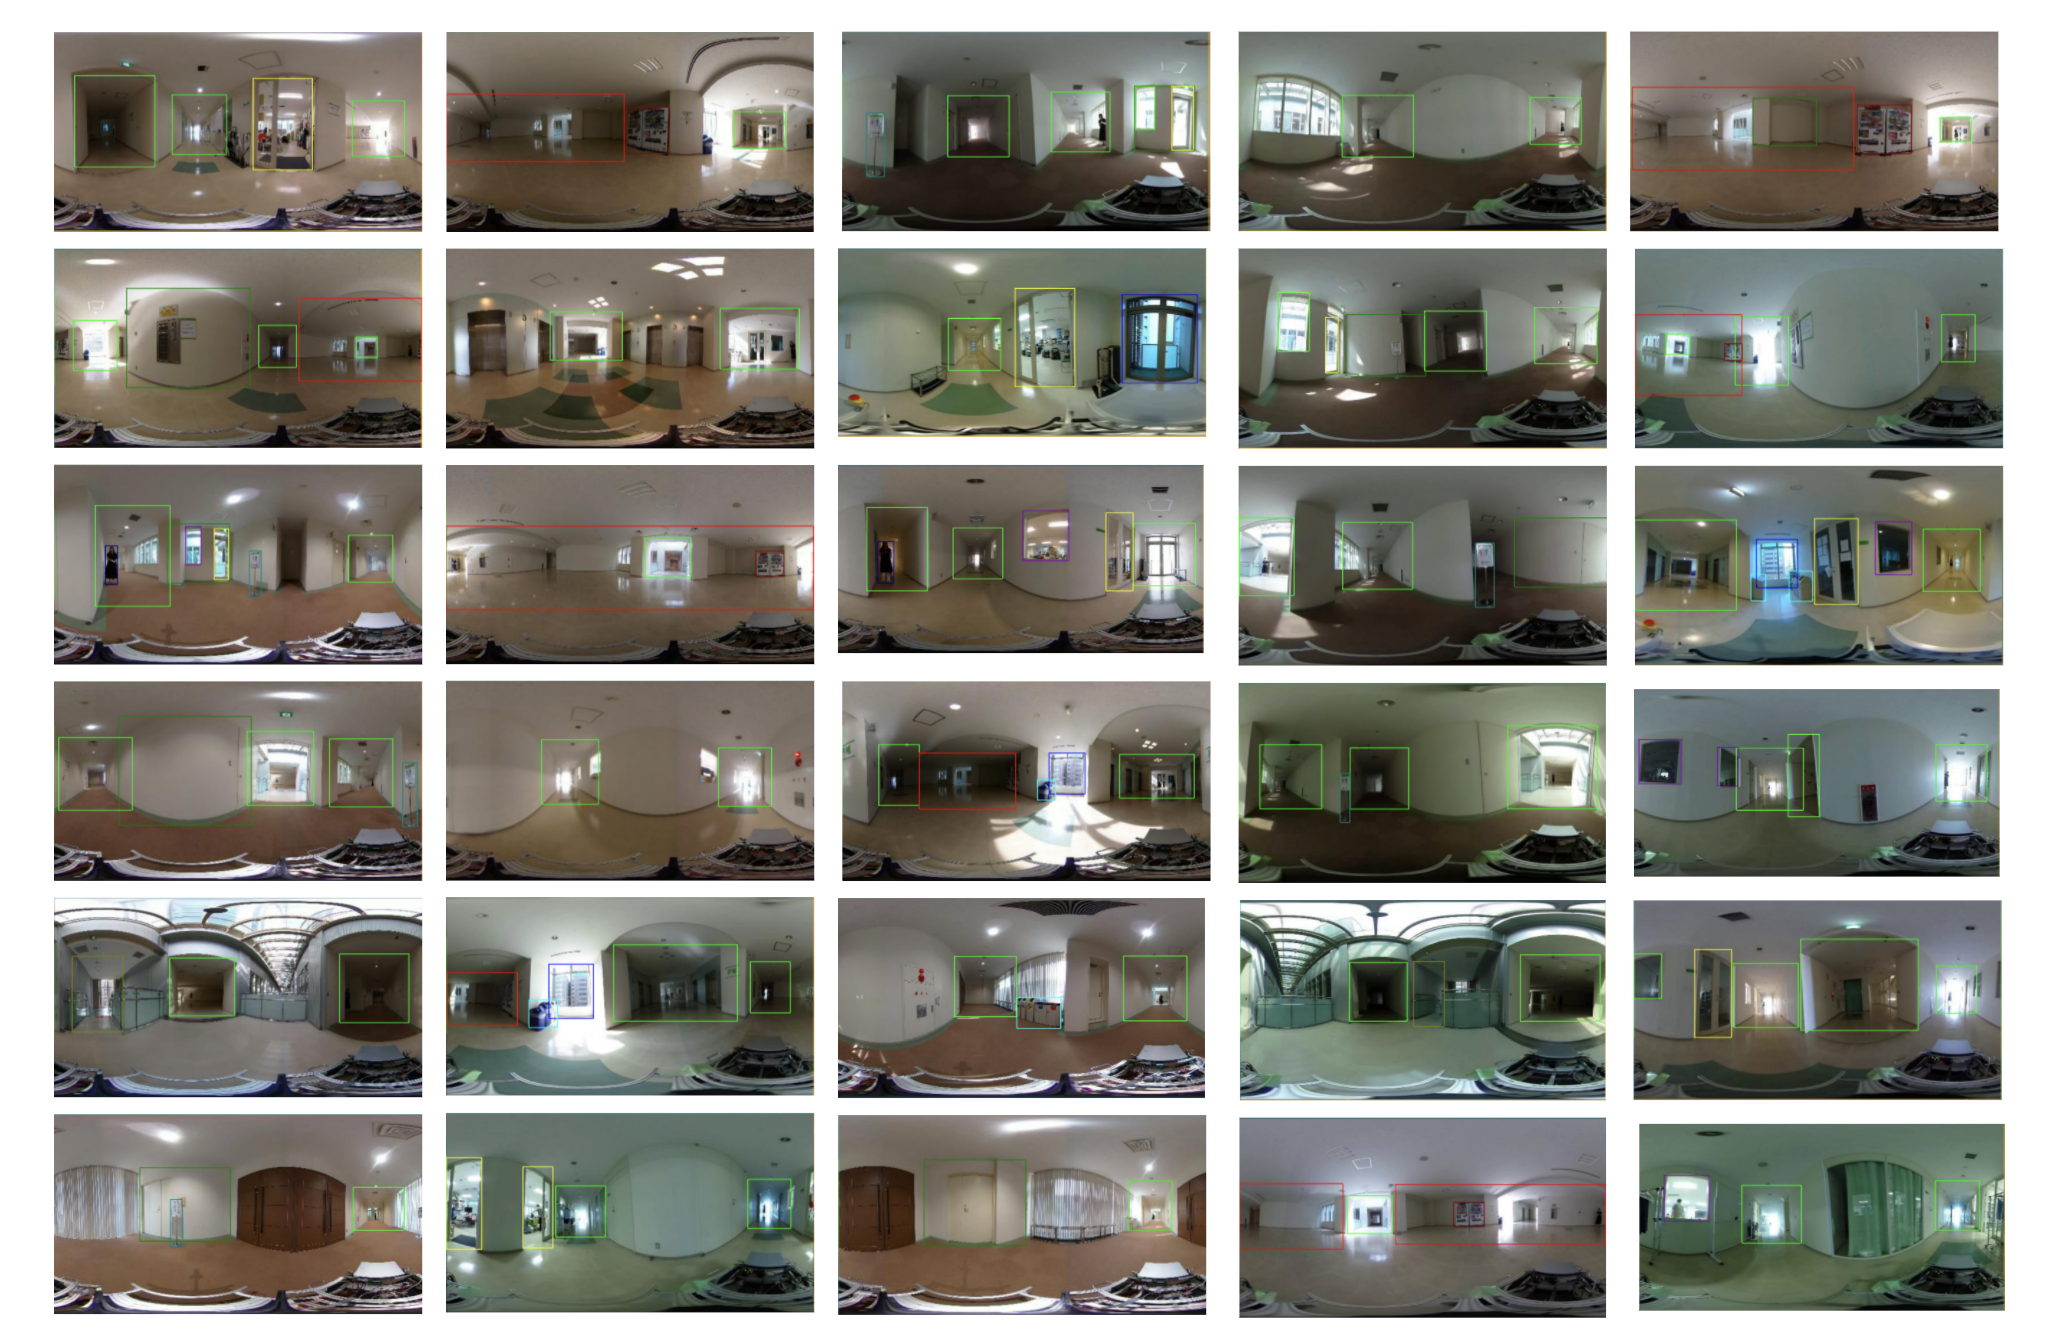
\includegraphics[width=10cm]{../images/dataset_exp.png}
         \caption{An example of a dataset.}
         \label{figure::dataset_fig}
        \end{figure}

        %データセットのクラス数
        \begin{table}[H]
            \caption{Class name to be labeled.}
            \centering
            \label{table::datasets_table}
            \begin{tabular}{lllll}
            \hline
            name of the class &  &  &  &  \\ 
            \hline \hline
            aisle             &  &  &  &  \\
            end               &  &  &  &  \\
            door\_end         &  &  &  &  \\
            human             &  &  &  &  \\
            door              &  &  &  &  \\
            step              &  &  &  &  \\
            square            &  &  &  &  \\
            vending\_machine  &  &  &  &  \\
            trash\_can        &  &  &  &  \\
            signboard         &  &  &  &  \\
            window            &  &  &  &  \\ 
            \hline
            \end{tabular}
        \end{table}
\end{document}

%\begin{figure}[H]
        %\centering  
        %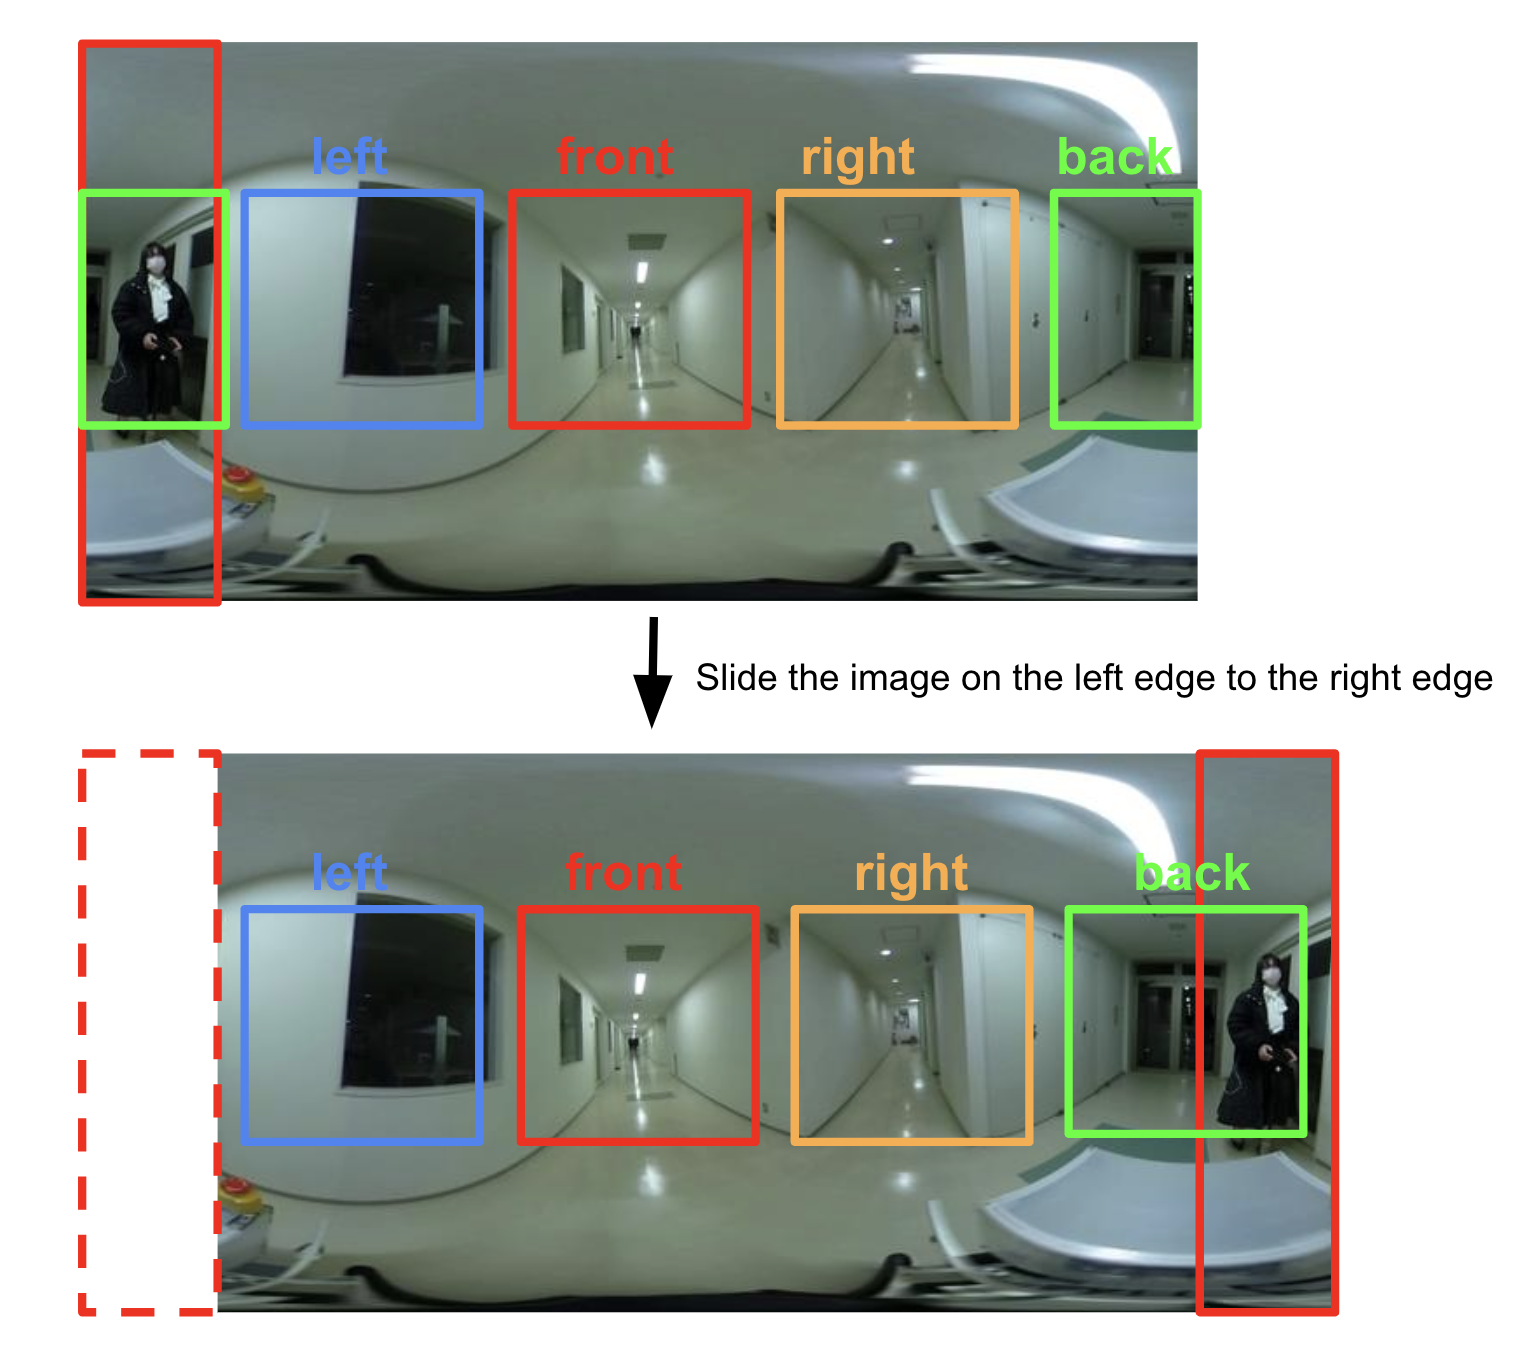
\includegraphics[width=10cm]{../images/image_proc2.png}
        %\caption{Preprocessing of spherical camera images.}
        %\label{figure::image_proc_fig}
        %\end{figure}